
\chapter{Software Architektur}
\section{Anforderungen}
\label{sec:Anforderungen} 
%Christoph
- nutzen der AR.Drone 2.0
- Vorgängerprojekt in Simulation nutzbar machen
 -> Problematik Windows -> Ubuntu
 1) Fliegen in Simulation mit Tastatur 
 2) Fliegen in Simulation mit Kinect Steuerung
 ggf. 3) Fliegen in Simulation mit Kinect + VR
- Projekt REMODE mit SVO von Davide Scaramuzza verwenden, um aus Bildern Tiefenbilder zu generieren
-> Bilder sollen sowohl von der realen Drohne kommen können, als auch aus einer simulierten Drohne
- Ziel: Forschung, ob man das Projekt nutzen kann, um ein Assistenzsystem zu entwickeln
	-> Wände / Türen erkennen
	-> aktives eingreifen der Drohne in das Geschehen -> Kollisionsvermeidung
	


\section{Überblick}
\label{Überblick}

\section{Implementation}
\label{Implementation}

\newpage
\subsection{Kamerakalibrierung}
\subsection{SVO}
\subsection{REMODE}
\subsection{Featureerkennung}

%\begin{figure}[ht]
%	\centering
%	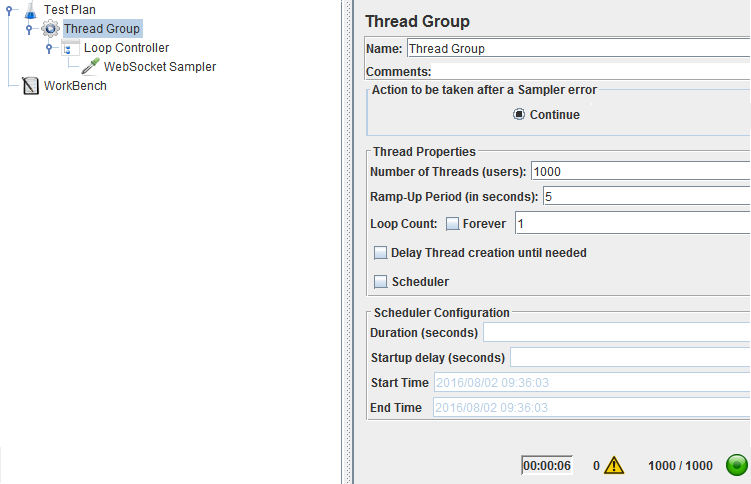
\includegraphics[scale=0.7]{Bilder/jMeterReal.png}
%	\caption[Testing with jMeter]{jMeter testing}
% 	\label{fig:testing}
%\end{figure}


